% Options for packages loaded elsewhere
\PassOptionsToPackage{unicode}{hyperref}
\PassOptionsToPackage{hyphens}{url}
%
\documentclass[
]{article}
\usepackage{amsmath,amssymb}
\usepackage{lmodern}
\usepackage{iftex}
\ifPDFTeX
  \usepackage[T1]{fontenc}
  \usepackage[utf8]{inputenc}
  \usepackage{textcomp} % provide euro and other symbols
\else % if luatex or xetex
  \usepackage{unicode-math}
  \defaultfontfeatures{Scale=MatchLowercase}
  \defaultfontfeatures[\rmfamily]{Ligatures=TeX,Scale=1}
\fi
% Use upquote if available, for straight quotes in verbatim environments
\IfFileExists{upquote.sty}{\usepackage{upquote}}{}
\IfFileExists{microtype.sty}{% use microtype if available
  \usepackage[]{microtype}
  \UseMicrotypeSet[protrusion]{basicmath} % disable protrusion for tt fonts
}{}
\makeatletter
\@ifundefined{KOMAClassName}{% if non-KOMA class
  \IfFileExists{parskip.sty}{%
    \usepackage{parskip}
  }{% else
    \setlength{\parindent}{0pt}
    \setlength{\parskip}{6pt plus 2pt minus 1pt}}
}{% if KOMA class
  \KOMAoptions{parskip=half}}
\makeatother
\usepackage{xcolor}
\usepackage{graphicx}
\makeatletter
\def\maxwidth{\ifdim\Gin@nat@width>\linewidth\linewidth\else\Gin@nat@width\fi}
\def\maxheight{\ifdim\Gin@nat@height>\textheight\textheight\else\Gin@nat@height\fi}
\makeatother
% Scale images if necessary, so that they will not overflow the page
% margins by default, and it is still possible to overwrite the defaults
% using explicit options in \includegraphics[width, height, ...]{}
\setkeys{Gin}{width=\maxwidth,height=\maxheight,keepaspectratio}
% Set default figure placement to htbp
\makeatletter
\def\fps@figure{htbp}
\makeatother
\setlength{\emergencystretch}{3em} % prevent overfull lines
\providecommand{\tightlist}{%
  \setlength{\itemsep}{0pt}\setlength{\parskip}{0pt}}
\setcounter{secnumdepth}{-\maxdimen} % remove section numbering
\ifLuaTeX
  \usepackage{selnolig}  % disable illegal ligatures
\fi
\IfFileExists{bookmark.sty}{\usepackage{bookmark}}{\usepackage{hyperref}}
\IfFileExists{xurl.sty}{\usepackage{xurl}}{} % add URL line breaks if available
\urlstyle{same} % disable monospaced font for URLs
\hypersetup{
  pdftitle={DISCRETE MATH MID},
  hidelinks,
  pdfcreator={LaTeX via pandoc}}

\title{DISCRETE MATH MID}
\author{}
\date{}

\begin{document}
\maketitle

\hypertarget{set-theory}{%
\section{SET THEORY}\label{set-theory}}

\begin{itemize}
\item
  A set is a collection of objects called elements.

\begin{verbatim}
$\{1, 2, 3\} = A$
Copy
\end{verbatim}
\item
  Sets can be \texttt{finite} or \texttt{infinite}\\
  {\(A = \{ 1,2,3,4,5,6,7,8,9\}\)}\\
  {\(Z = \{ 1,2,3,4,...\}\)}
\end{itemize}

Additional Points:

\begin{itemize}
\tightlist
\item
  Repeated elements are listed once\\
  {\(\{ a,b,a,c,b,a\} = \{ a,b,c\}\)}
\item
  {There is \textbf{NO ORDER} in a set.}\\
  {\(\{ 3,2,1\} = \{ 1,2,3\}\)}\\
  {\(= \{ 2,1,3\}\)}
\end{itemize}

\hypertarget{common-sets}{%
\subparagraph{Common Sets}\label{common-sets}}

\begin{itemize}
\tightlist
\item
  Natural Numbers\\
  {\[N = \{ 0,1,2,3,...\}\]} {\[OR\]} {\[\{ 1,2,3,...\}\]}
\item
  Integers\\
  {\[Z = \{..., - 2, - 1,0,1,2,...\}\]}
\item
  Rational Numbers\\
  {\[Q = \{\frac{1}{1},\frac{1}{2},\frac{1}{3},\frac{2}{3}\}\]}
\end{itemize}

\hypertarget{elements-and-cardinality}{%
\subsection{Elements and Cardinality}\label{elements-and-cardinality}}

{Cardinality (size)}

Let {\(C = \{ yellow,blue,red\}\)}

{Yellow} is an element of \texttt{C}

\begin{quote}
{\[Yellow \in C\]}
\end{quote}

{Green} is not an element of \texttt{C}

\begin{quote}
{\[Green \notin C\]}
\end{quote}

The cardinality(size) of \texttt{C\ is\ 3}

\begin{quote}
{\[|C| = 3\]}
\end{quote}

\hypertarget{the-empty-set}{%
\subsection{The Empty Set}\label{the-empty-set}}

The Empty Set symbol:

\begin{quote}
{\(\phi = \{\}\)}
\end{quote}

It is the only set that has a size of 0

\begin{quote}
{\(|\phi| = 0\)}
\end{quote}

but, What is the size of a \textbf{set} containing {the Empty Set} ?

\begin{quote}
{\(|\{\varnothing\}| = 1\)}
\end{quote}

The answer is 1, because the BIG SET has 1 element.

BUT, it\textquotesingle s different to the set that contains
\textbf{NOTHING}.

\begin{quote}
{\(|\{\}| = 0\)}
\end{quote}

\hypertarget{set-builder-notation}{%
\subsection{Set-Builder Notation}\label{set-builder-notation}}

\begin{enumerate}
\tightlist
\item
  {\(\cdot \mathbb{Q} = \{\ldots,1/1,1/2,1/3,2/3,\ldots\}\)}
\end{enumerate}

{\[= \left\{ \frac{m}{n} \mid m,n \in \mathbb{Z},n \neq 0 \right\}\]}

\begin{enumerate}
\setcounter{enumi}{1}
\tightlist
\item
  {\(2\mathbb{Z} = \{\ldots, - 4, - 2,0,2,4,\ldots\}\)}
\end{enumerate}

{\[\left\{ 2n \mid \begin{array}{l}
{n \in \mathbb{Z}} \\
\end{array} \right\}\]}

\begin{enumerate}
\setcounter{enumi}{2}
\tightlist
\item
  \texttt{Desk\ =\ \{drink,\ laptop,\ microphone\}}\strut \\
  {\[= \{ x \mid x\; is\; on\; my\; desk\}\]}
\end{enumerate}

\hypertarget{example}{%
\subsubsection{Example:}\label{example}}

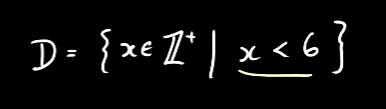
\includegraphics[width=3.125in,height=\textheight]{C:/Users/johnr/OneDrive/Obsidian Vault/Pasted image 20221107111639.png}\\
List the elements of D.\\
{\[1,2,3,4,5\]}

What is the cardinality of D?\\
{\[|D| = 5\]}What is the cardinality of
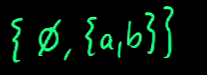
\includegraphics[width=1.5625in,height=\textheight]{C:/Users/johnr/OneDrive/Obsidian Vault/Pasted image 20221107111838.png}\\
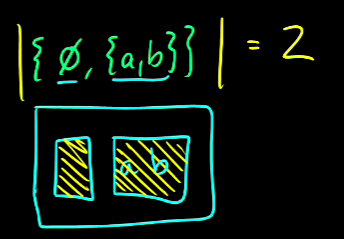
\includegraphics[width=3.38542in,height=\textheight]{C:/Users/johnr/OneDrive/Obsidian Vault/Pasted image 20221107112051.png}\\
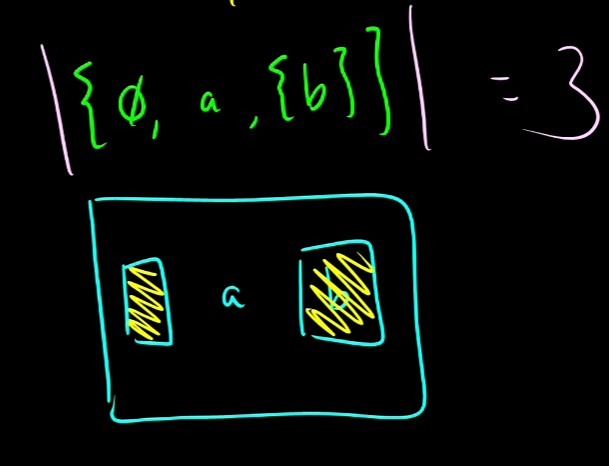
\includegraphics[width=3.38542in,height=\textheight]{C:/Users/johnr/OneDrive/Obsidian Vault/Pasted image 20221107112243.png}

\hfill\break
\hfill\break

\hypertarget{relations-and-functions}{%
\section{RELATIONS and FUNCTIONS}\label{relations-and-functions}}

\hfill\break

\hypertarget{relations-of-relations}{%
\subsubsection{Relations of relations}\label{relations-of-relations}}

\begin{itemize}
\tightlist
\item
  \textbf{Reflexive} - For all \texttt{X}, we have \texttt{xRx} or it
  means \texttt{X} is related to itself.\\
  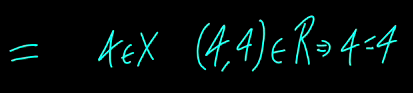
\includegraphics[width=3.125in,height=\textheight]{C:/Users/johnr/OneDrive/Obsidian Vault/Pasted image 20221107185455.png}
\item
  \textbf{Symmetric} - For all elements \texttt{X} and elements
  \texttt{Y}, if \texttt{X} is related to \texttt{Y} then \texttt{Y} is
  related to \texttt{X}\\
  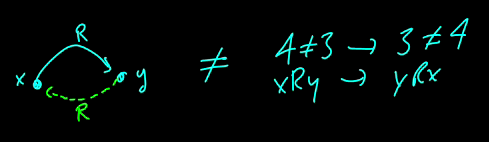
\includegraphics[width=3.125in,height=\textheight]{C:/Users/johnr/OneDrive/Obsidian Vault/Pasted image 20221107185540.png}
\item
  \textbf{Transitive} - For 3 elements \texttt{X,Y} and \texttt{Z}, If
  \texttt{X} is related to \texttt{Y} and \texttt{Y} is related to
  \texttt{Z\ }then \texttt{X} is also related to \texttt{Z}.\\
  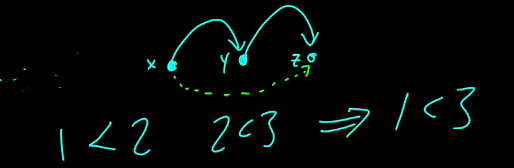
\includegraphics[width=3.125in,height=\textheight]{C:/Users/johnr/OneDrive/Obsidian Vault/Pasted image 20221107185908.png}
\end{itemize}

\hypertarget{functions}{%
\subsubsection{Functions}\label{functions}}

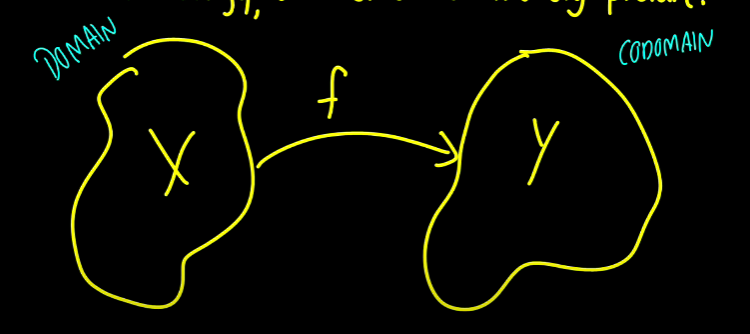
\includegraphics[width=3.125in,height=\textheight]{C:/Users/johnr/OneDrive/Obsidian Vault/Pasted image 20221108093142.png}\\
This function maps an element of \texttt{X} into an element of
\texttt{Y},\\
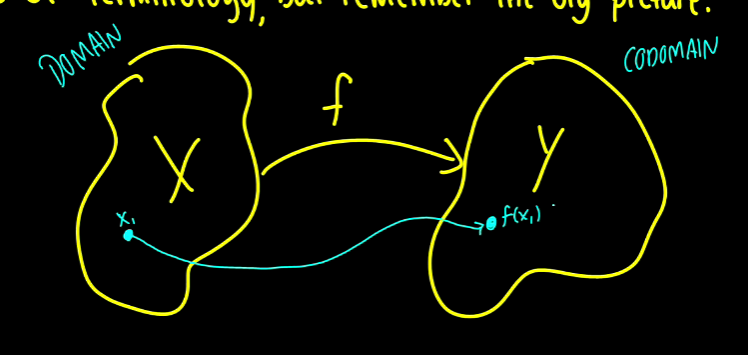
\includegraphics[width=3.125in,height=\textheight]{C:/Users/johnr/OneDrive/Obsidian Vault/Pasted image 20221108093227.png}\\
Which we will call it \texttt{Y1}\\
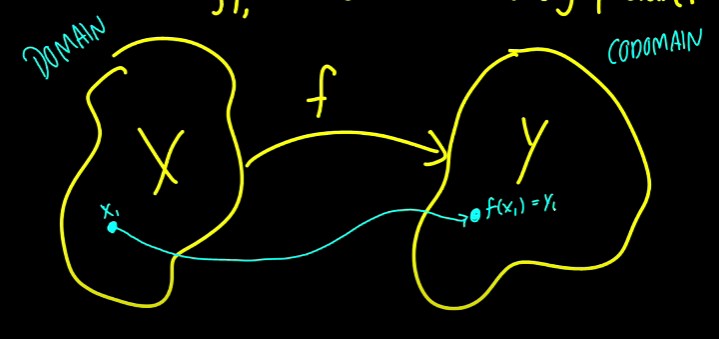
\includegraphics[width=3.125in,height=\textheight]{C:/Users/johnr/OneDrive/Obsidian Vault/Pasted image 20221108093248.png}\\
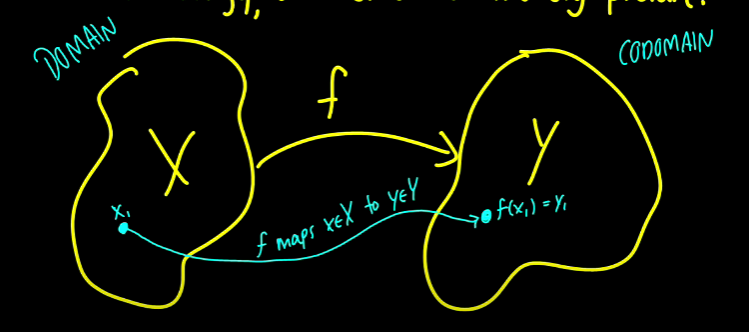
\includegraphics[width=5.20833in,height=\textheight]{C:/Users/johnr/OneDrive/Obsidian Vault/Pasted image 20221108093439.png}\\
Wherever we put the elements in \texttt{X} it will always be maps to
\texttt{Y} and what we call the \texttt{Y} is \textbf{RANGE}.\\
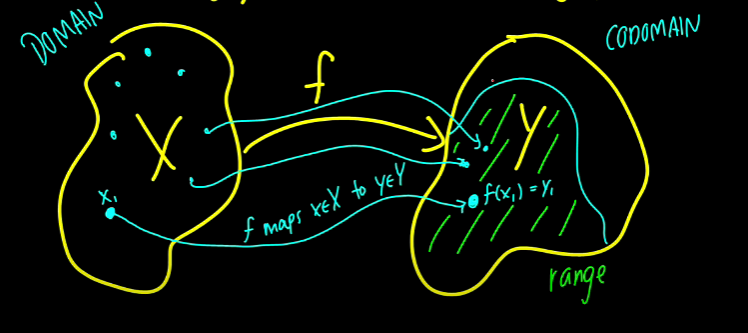
\includegraphics[width=3.64583in,height=\textheight]{C:/Users/johnr/OneDrive/Obsidian Vault/Pasted image 20221108093703.png}\\
The \texttt{REDZONE} here is part of the CODOMAIN but is not part of the
RANGE\\
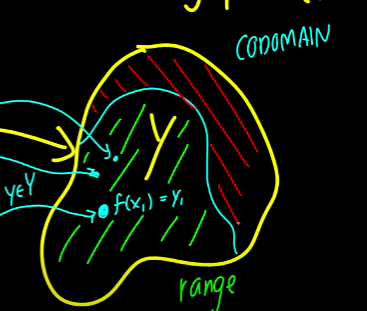
\includegraphics[width=3.125in,height=\textheight]{C:/Users/johnr/OneDrive/Obsidian Vault/Pasted image 20221108093805.png}

\hypertarget{domain-and-range}{%
\subsection{Domain and Range}\label{domain-and-range}}

The~\textbf{domain and range}~are defined for
a~\href{https://www.cuemath.com/algebra/relations-in-math/}{relation}~and
they are the sets of all the x-coordinates and all the y-coordinates of
ordered pairs respectively. For example, if the relation is, R = \{(1,
2), (2, 2), (3, 3), (4, 3)\}, then:

\begin{itemize}
\tightlist
\item
  Domain = the set of all x-coordinates = \{1, 2, 3, 4\}
\item
  Range = the set of all y-coordinates = \{2, 3\}
\end{itemize}

We can visualize this here:

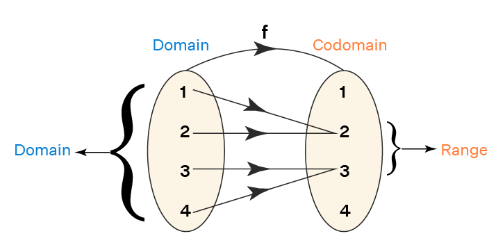
\includegraphics{C:/Users/johnr/OneDrive/Obsidian Vault/Pasted image 20221108111351.png}

\begin{itemize}
\item
  DOMAIN - all of the first values (\texttt{X} coordinates)
\item
  RANGE - all of the second values (\texttt{Y} coordinates)
\item
  CONTINUOS GRAPHS - Graphs with \texttt{CONNECTED\ LINES} or
  \texttt{CURVES} (includes values that are not integers)
\item
  DISCRETE GRAPHS - Graph that contains \texttt{POINTS} that are only
  Integers. \textbf{There is not a line connecting the points}.
\end{itemize}

\hfill\break
\hfill\break

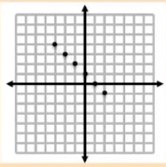
\includegraphics{C:/Users/johnr/OneDrive/Obsidian Vault/Pasted image 20221108095315.png}\\
DISCRETE GRAPH

\begin{itemize}
\tightlist
\item
  Domain: X\\
  \texttt{\{-3,\ -2,\ -1,\ 0,\ 1,\ 2\}}
\item
  Range: Y\\
  \texttt{\{4,\ 3,\ 2,\ 1,\ 0,\ -1\}}
\end{itemize}

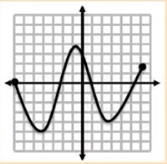
\includegraphics{C:/Users/johnr/OneDrive/Obsidian Vault/Pasted image 20221108095506.png}\\
CONTINUOS GRAPH

\begin{itemize}
\tightlist
\item
  Domain: X\\
  \texttt{-7,\ ≤\ x\ ≤\ 6}
\item
  Range: Y\\
  \texttt{-5\ ≤\ y\ ≤\ 4}
\end{itemize}

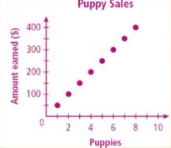
\includegraphics{C:/Users/johnr/OneDrive/Obsidian Vault/Pasted image 20221108095806.png}\\
DISCRETE GRAPH

\begin{itemize}
\tightlist
\item
  Domain: X\\
  \texttt{\{1\ ,\ 2,\ 3,\ ...\ ,\ 9\}}
\item
  Range: Y\\
  \texttt{\{50,\ 100,\ 150,\ ...\ ,\ 400\}}
\end{itemize}

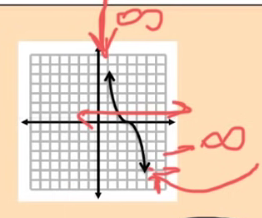
\includegraphics{C:/Users/johnr/OneDrive/Obsidian Vault/Pasted image 20221108100036.png}\\
CONTINUOUS GRAPH

\begin{itemize}
\tightlist
\item
  Domain: X\\
  \texttt{All\ Real\ Numbers\ (ARN)\ or\ -∞\ ≤\ X\ ≤\ ∞}
\item
  Range: Y\\
  \texttt{All\ Real\ Numbers\ (ARN)\ or\ -∞\ ≤\ Y\ ≤\ ∞}
\end{itemize}

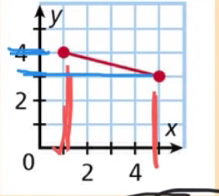
\includegraphics{C:/Users/johnr/OneDrive/Obsidian Vault/Pasted image 20221108100506.png}\\
CONTINUOUS GRAPH

\begin{itemize}
\tightlist
\item
  Domain: X\\
  \texttt{1\ ≤\ X\ ≤\ 5}
\item
  Range: Y\\
  \texttt{3\ ≤\ Y\ ≤\ 4}
\end{itemize}

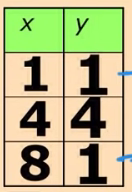
\includegraphics{C:/Users/johnr/OneDrive/Obsidian Vault/Pasted image 20221108100724.png}\\
DISCRETE

\begin{itemize}
\tightlist
\item
  Domain: X\\
  \texttt{\{1,\ 4,\ 8\}}
\item
  Range: Y\\
  \texttt{\{1,\ 4\}}
\end{itemize}

\hypertarget{domain-and-range-of-function}{%
\subsection{Domain and Range of
Function}\label{domain-and-range-of-function}}

The~\textbf{domain and range of a function}~are the components of
a~\href{https://www.cuemath.com/calculus/What-are-functions/}{function}.
The domain is the set of all the input values of a function and range is
the possible output given by the function. Domain→ Function →Range. If
there exists a function f: A →B such that every element of A is mapped
to elements in B, then A is the domain and B is the co-domain. The image
of an element \textquotesingle a\textquotesingle{} under a relation R is
given by \textquotesingle b\textquotesingle, where (a,b) ∈ R. The range
of the function is the set of images. The domain and range of a function
is denoted in general as follows: Domain(f) = \{x ∈ R\} and
range(f)=\{f(x) : x ∈ domain(f)\}

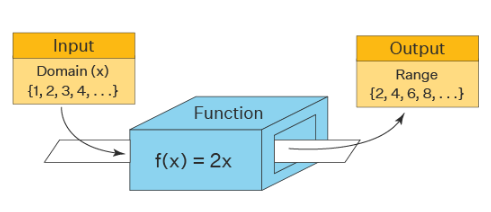
\includegraphics{C:/Users/johnr/OneDrive/Obsidian Vault/Pasted image 20221108111524.png}\\
The domain and range of this function f(x) = 2x is given as domain D
=\{x ∈ N \} , range R = \{(y): y = 2x\}

\hypertarget{algebra-of-function}{%
\subsection{Algebra of Function}\label{algebra-of-function}}

If \texttt{f} and \texttt{g} are functions, and \texttt{X} is an element
of the domain of each function, then\\
{\[(f + g)(x) = f(x) + g(x)\]}{\[(f - g)(x) = f(x) - g(x)\]}{\[(f \ast g)(x) = f(x) \ast g(x)\]}{\[(\frac{f}{g})(x) = f\frac{x}{g(x)},g(x) \neq 0\]}

EXAMPLES:\\
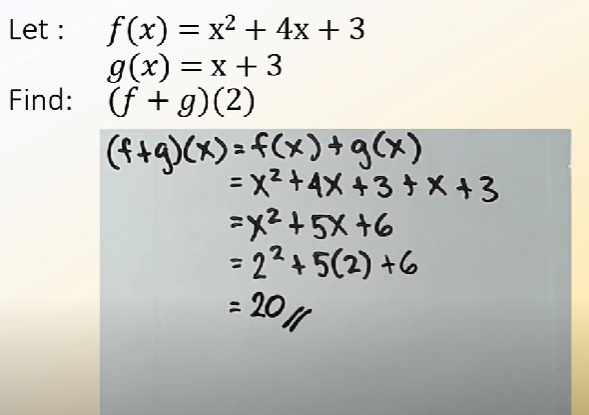
\includegraphics[width=3.125in,height=\textheight]{C:/Users/johnr/OneDrive/Obsidian Vault/Pasted image 20221108131407.png}\\
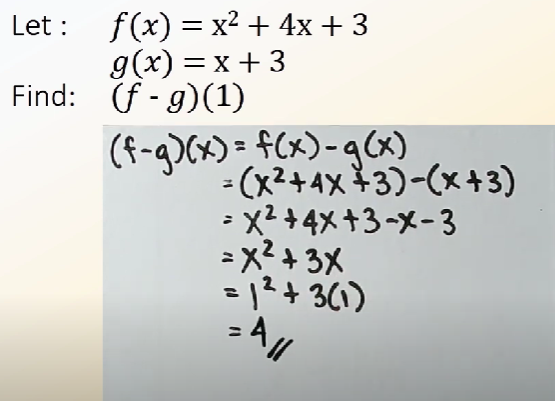
\includegraphics[width=3.125in,height=\textheight]{C:/Users/johnr/OneDrive/Obsidian Vault/Pasted image 20221108131423.png}\\
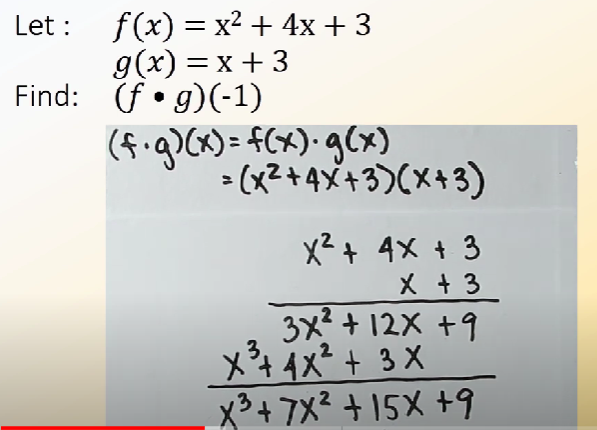
\includegraphics[width=3.125in,height=\textheight]{C:/Users/johnr/OneDrive/Obsidian Vault/Pasted image 20221108131444.png}\\
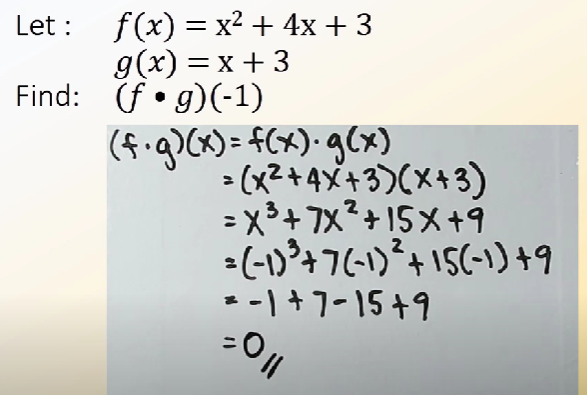
\includegraphics[width=3.125in,height=\textheight]{C:/Users/johnr/OneDrive/Obsidian Vault/Pasted image 20221108131503.png}\\
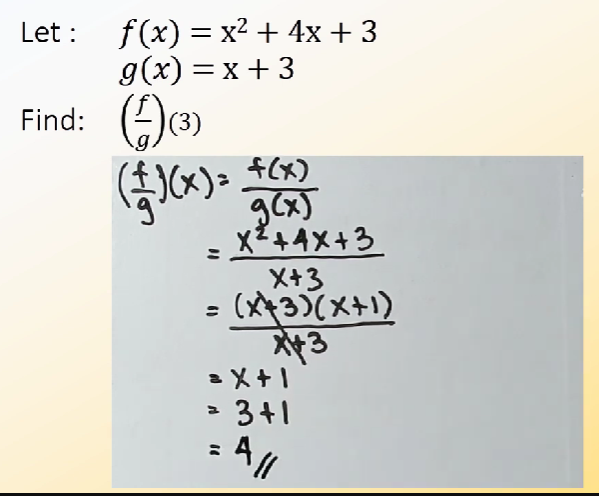
\includegraphics[width=3.125in,height=\textheight]{C:/Users/johnr/OneDrive/Obsidian Vault/Pasted image 20221108131541.png}

\hypertarget{addition}{%
\subsubsection{Addition}\label{addition}}

FORMULA : \textbf{\texttt{(f\ +\ g)\ (x)\ =\ f(x)\ +\ g(x)}}\\
\textbf{Example:}~\\
When f(x) = x2~+ 2 and\\
g(x) = x + 1, then

(f + g)(x) = \texttt{f(x)\ +\ g(x)}

= \texttt{x2~+\ 2\ +\ x\ +\ 1}

=\texttt{\ x2~+\ x\ +\ 3}

\hypertarget{subtraction}{%
\subsubsection{Subtraction}\label{subtraction}}

FORMULA: \textbf{\texttt{(f\ -\ g)\ (x)\ =\ f(x)\ -\ g(x)}}\\
\textbf{Example:}~When f(x) = x2~+ 2 and\\
g(x) = x + 1, then

(f - g)(x) = \texttt{f(x)\ -\ g(x)}

= \texttt{x2~+\ 2\ -\ (x\ +\ 1)}

= \texttt{x2~-\ x\ +\ 1}

\hypertarget{multiplication}{%
\subsubsection{Multiplication}\label{multiplication}}

FORMULA: \textbf{\texttt{(f\ ·\ g)\ (x)\ =\ f(x)\ ·\ g(x)}}\\
\textbf{Example:}~When f(x) = x2~+ 2 and\\
g(x) = x + 1, then

(f · g)(x) =\texttt{\ f(x)\ ·\ g(x)}

= \texttt{(x2~+\ 2)\ ·\ (x\ +\ 1)}

= \texttt{x3~+\ x2~+\ 2x\ +\ 2}

\hypertarget{division}{%
\subsubsection{Division}\label{division}}

FORMULA :
\textbf{\texttt{\ (f\ /\ g)\ (x)\ =\ f(x)\ /\ g(x),\ given\ g(x)\ ≠\ 0}}

\textbf{Example:}~When f(x) = x2~+ 2\\
and g(x) = x + 1, then

(f / g)(x) =\texttt{\ f(x)\ /\ g(x)}

= \texttt{(x2~+\ 2)\ /\ (x\ +\ 1)}\\
Since the domain of each of f(x) is the set of all real numbers, R; and
the domain of g(x) is the set of all real numbers except -1 (as x + 1 is
in the denominator, x + 1 ≠ 0 ⇒ x ≠ -1). So the domain of (f / g)(x) is
R - \{-1\}.

\textbf{Important Notes on Algebra of Functions:}

For any two functions f(x) and g(x):

\begin{itemize}
\tightlist
\item
  (f + g) (x) = \texttt{f(x)\ +\ g(x)}
\item
  (f - g) (x) = \texttt{f(x)\ -\ g(x)}
\item
  (f · g) (x) = \texttt{f(x)\ ·\ g(x)}
\item
  (f / g) (x) = \texttt{f(x)\ /\ g(x),\ g(x)\ ≠\ 0}
\end{itemize}

\hypertarget{inverse-function}{%
\subsection{Inverse Function}\label{inverse-function}}

Function will only Intersect the VERTICAL line once on any part of its
graph.\\
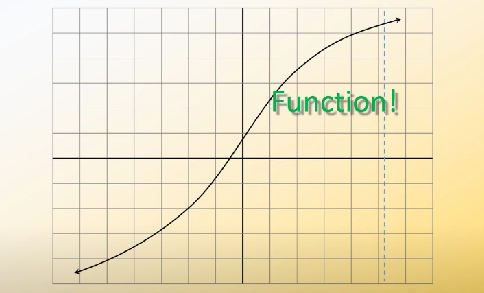
\includegraphics[width=3.125in,height=\textheight]{C:/Users/johnr/OneDrive/Obsidian Vault/Pasted image 20221108134647.png}\\
If It intersect multiple times then it is NOT A FUNCTION\\
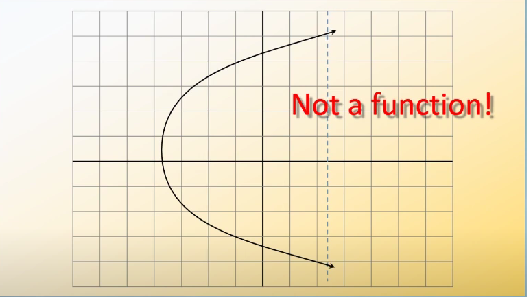
\includegraphics[width=3.125in,height=\textheight]{C:/Users/johnr/OneDrive/Obsidian Vault/Pasted image 20221108134633.png}

The inverse of f(x) is f-1(x)

EXAMPLE:\\
\textbf{\texttt{f(x)\ =\ 3x\ +\ 6}}\strut \\
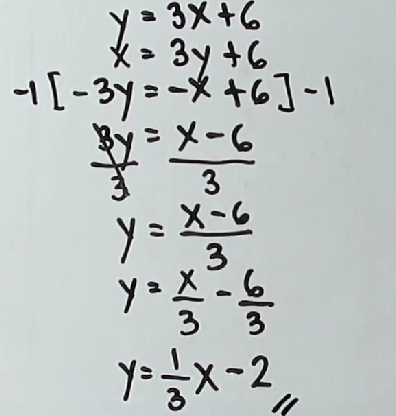
\includegraphics[width=3.125in,height=\textheight]{C:/Users/johnr/OneDrive/Obsidian Vault/Pasted image 20221108134901.png}

\end{document}
